\chapter{Fairness}

\qs{}{Che cos'è l'IA?}

\paragraph{Un sistema IA può essere inteso come:}

\begin{itemize}
  \item \fancyglitter{Dati:} esperienza di input presa in considerazione. 
  \item \fancyglitter{Algoritmi:} mezzo per elaborare i dati. 
  \item \fancyglitter{Decisioni:} che possiamo impiegare direttamente o utilizzare come assistenza. 
\end{itemize}

\nt{Per esempio, per Russell e Norvig, il termostato è un esempio di IA.}

\qs{}{Come si può sapere se questo sistema è \fancyglitter{affidabile}?}

\section{Introduzione alla Fairness}

Si può concordare che uno strumento è affidabile se commette un numero limitato di errori, ossia quando è in grado di seguire in modo accurato alle nostre istruzioni. Spesso non è semplice capirlo, esistono due possibili approcci:

\begin{itemize}
  \item \fancyglitter{Metodo Clinico:} il decisore combina o elabora le informazioni nella sua mente. Un metodo IA clinico si basa su una serie di regole prestabilite fornite da un esperto del settore. 
  \item \fancyglitter{Metodo Attuariale o Statistico:} le conclusioni si basano esclusivamente su relazioni empiricamente stabilite tra i dati e la condizione o l'evento di interesse. Un metodo IA attuariale esami i dati passati per prevedere i risultati futuri. 
\end{itemize}

\nt{Grosso modo si sono effettuati metodi clinici dal 1956 al 1990, mentre dal 1980 a oggi si sono sviluppati sistemi attuariali.}

\subsection{Metodo Clinico vs. Metodo Attuariale}

\dfn{Sistemi Esperti}{
  I sistemi esperti hanno rappresentato un'applicazione incredibilmente risucita dell'IA (metodo clinico): se si raccoglie una quantità sufficiente di conoscenze, è possibile costruire una catena di regole che offrono buone prestazioni per un determinato compito.
}

\begin{figure}[h]
    \centering
    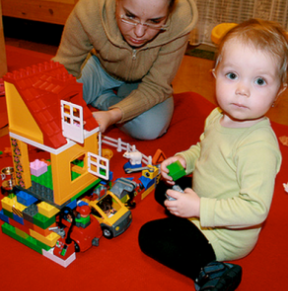
\includegraphics[scale=0.45]{04P/lego.png}
    \caption{Immagine di bambino con mattoncini.}
    \label{fig:mat}
\end{figure}

\qs{}{Cosa si vede nell'immagine \ref{fig:mat}?}

\begin{itemize}
  \item Per anni i ricercatori IA hanno considerato impossibile risolvere questo task con il metodo clinico, ossia definire cosa sia un "bambino" o un "mattoncino" in ogni circostanza. 
  \item Ai giorni nostri è possibile farlo.
  \item Le tecniche di \fancyglitter{apprendimento automatico} (IA attuarie) hanno compiuto progressi teorici e tecnologici. 
  \item Per questo è nata la necessità di sviluppare enormi quantità di dati.
  \item Negli anni dal 2010 in avanti le tecniche di \fancyglitter{deep learning} hanno contribuito a migliorare questo processo.
  \item Le reti neurali hanno maggiore scalabilità rispetto a Hidden Markov Model, Modelli Gaussiani, Reti Bayesiane, etc.
\end{itemize}

\nt{CONTENT WARNING (TW: razzismo, sessismo, autolesionismo, suicidio, ideazione suicida). Saltare a \ref{sec:MLF}.}

\subsection{Esempi del Machine Learing}

\begin{itemize}
  \item Classificazione automatica delle immagini. 
  \item Google Photos tagga due afro-americani come gorilla con il suo software di riconoscimento facciale. 
  \item Un algoritmo IA utilizzato per concorsi di bellezza\footnote{Well i concorsi di bellezza sono intrinsecamente razzisti quindi non era effettivamente un'idea intelligente.}: ai modelli non piacciono le persone di pelle scura.
  \item Modelli di predizione dei crimini: per valutare un "livello di rischio". 
  \item I modelli di scraping AI mostrano una discriminazione nei confronti delle donne\footnote{Che sorpresa...} (fig: \ref{fig:bias}).
    \begin{figure}[h]
    \centering
    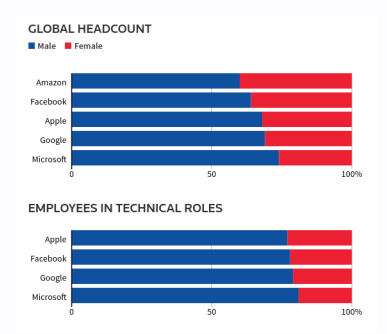
\includegraphics[scale=0.41]{04P/bias.png}
    \caption{Impiegati per sesso (rip NB representation).}
    \label{fig:bias}
\end{figure}
\item I modelli di Amazon avrebbero dovuto essere addestrati a osservare i modelli ricorrenti nei curriculum inviati all'azienda (che erano appunto uomini). 
\item Negli stati uniti le persone con un nome tipicamente bianco hanno più possibilità di essere chiamati per colloqui.
\item Un uomo belga si è suicidato dopo sei settimane di scambi con un chatbot.
\end{itemize}

\qs{}{Ma come è potuto succedere?}

\begin{itemize}
  \item Gli algoritmi sono sessisti/razzisti? 
  \item Chi è il responsabile?
  \item Come hanno fatto gli ingegneri a non notare questi problemi prima dell'implementazione? 
  \item È illegale?
\end{itemize}

\paragraph{Problema:}

\begin{itemize}
  \item L'IA attuariale è spesso \fancyglitter{opaca}: è difficile capire perché un determinato sistema di IA ha preso una particolare decisione. 
  \item Nonostante sia possibile ispezionare i parametri di un modello (il suo algoritmo) collegarli a delle ragioni per cui sono state prese effettivamente delle decisioni. 
\end{itemize}

\section{Machine Learning e Fairness}
\label{sec:MLF}

\dfn{Apprendimento}{
  Si dice che un programma per computer apprende dall'esperienza $E$ rispetto a una classe di compiti $T$ e a una misura di prestazione $P$ se la sua prestazione nei compiti in $T$, misurata da $P$, migliora con l'esperienza $E$.
}

\paragraph{Tasks comuni nel ML:}

\begin{itemize}
  \item \fancyglitter{Classificazione:} dati alcuni dati su entità del mondo reale e un insieme di etichette a essi applicabili, imparare ad assegnare tali etichette a entità non viste. 
  \item \fancyglitter{Regressione:} dati alcuni dati su entità del mondo reale e un insieme di numeri reali a essi applicabili, imparare ad assegnare numeri a entità non viste.
\end{itemize}

\subsection{Classificazione}

\dfn{Classificazione}{
  \begin{itemize}
    \item $X$: dati, covariati. 
    \item $Y$: verità fondamentali, etichette, target variabili.
  \end{itemize}
  La classificazione è il processo che consiste nel determinare un valore plausibile per $Y$ dato $X$. Si cerca di apprendere i parametri $\theta$ di una funzione $f_\theta$ che mappa la variabile casuale $X$ su una stima $\hat Y$ di $Y$:

$$\hat Y = f_\theta (X)$$

}

\cor{Variabile Casuale}{
  Una variabile casuale è un dispositivo matematico utilizzato per descrivere quantità che dipendono da eventi casuali o che sono in generale incerte.
}

\nt{Esempi di variabili casuali: lancio di un dado o di una moneta.}

\begin{figure}[h]
    \centering
    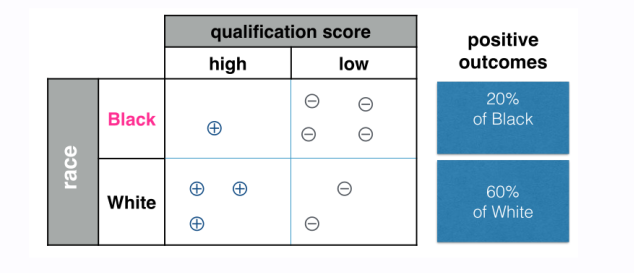
\includegraphics[scale=0.5]{04P/class.png}
    \caption{Esempio di classificazione.}
\end{figure}

\clm{}{}{
  \begin{itemize}
    \item Il processo di apprendimento dei parametri per $f_\theta$ dipende dall'algoritmo e dalla scelta della rappresentazione. 
    \item Per la regressione logistica $\theta$ è un vettore di valori reali la cui lunghezza è uguale $X + 1$ dove $X$ è il numero di colonne. 
    \item La rappresentazione più naturale per $\theta$ può essere diversa se cerchiamo di apprendere un albero decisionale. 
  \end{itemize}
}

\dfn{Accuratezza di un Classificatore}{
  Se $P(Y = f_\theta (X)) = P(Y = \hat Y) = 1$ si ha il classificatore perfetto. In generale $P(Y = \hat Y)$ è l'accuratezza del classificatore.
}

\paragraph{In alcuni casi l'accuratezza potrebbe non essere utile:}

\begin{itemize}
  \item Si vuole prevedere se il prossimo anno si verificherà una pandemia. 
  \item Negli ultimi 2000 anni si sarebbe potuta prevedere una probabilità del 99\% di no. 
  \item Questo mostra che è necessario avere altri modi per descrivere le \fancyglitter{prestazioni del classificatore}.
\end{itemize}

\cor{Costo}{
  Il costo è il numero reale $l(\hat y, y)$ che otteniamo quando classifichiamo un esempio con etichetta $y$ come $\hat y$.
}

\dfn{Classificatore Ottimale}{
Il classificatore ottimale è il classificatore che minimizza 

$$\bbE(l(Y, \hat Y))$$ 

dove $\bbE$ è il valore atteso. 

}

\nt{Due classificatori possono avere la stessa accuratezza ma avere costi differenti.}

\cor{Errore di Classificazione}{
  Il classificatore ottimale che riduce al minimo l'errore di classificazione soddisfa la seguente proprietà: 

$$\hat{Y} = f(X), \quad \text{dove } f(X) = 
\begin{cases}
1 & \text{se } \mathbb{P}(Y = 1 \mid X = x) > \frac{1}{2} \\
0 & \text{altrimenti}
\end{cases}
$$

}

\nt{Si può ottenere un classificatore ottimale da alcuni valori di probabilità scegliendo la soglia giusta.}

\paragraph{Problemi:}

\begin{itemize}
  \item Tasso di falsi positivi sbilanciato. 
  \item Disparità nei risultati positivi.
\end{itemize}

\subsection{Il Ciclo ML}

\qs{}{Cosa succede nell'apprendimento automatico prima e dopo l'addestramento di un classificatore?}

\begin{figure}[h]
    \centering
    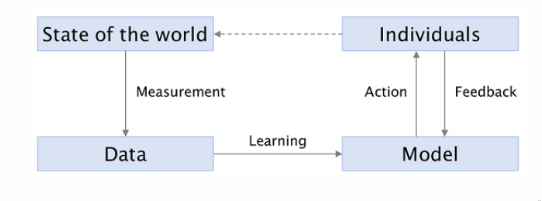
\includegraphics[scale=0.5]{04P/ciclo ML.png}
    \caption{Ciclo del ML.}
\end{figure}

\begin{itemize}
  \item \fancyglitter{Apprendimento:} il processo di ricerca di buoni parametri $\theta$ per $f$ e, possibilmente, di una soglia ottimale.
  \item \fancyglitter{Azioni:} come vengono impiegate le decisioni del nostro modello su input nuovi e mai visti prima. 
  \item \fancyglitter{Esempi:} eliminare tutte le mail classificate come spam, decidere se una persona con un determinato punteggio di rischio può essere rilasciata su cauzione.
  \item \fancyglitter{Feedback:} facoltativamente registrare come gli utenti hanno reagito alle azioni intraprese.
  \item \fancyglitter{Misurazione:} il processo in cui lo stato del mondo viene ridotto a tabelle di dati.
\end{itemize}

\paragraph{Il processo di misurazione:}

\begin{itemize}
  \item Spesso nel ML è dato per scontato. 
  \item Vengono effettuate $N$ misurazioni su una proprietà osservabile $L$. 
  \item Il valore convergerà alla lunghezza vera quando $N \rightarrow \infty$. 
  \item Definizione alternativa: la $n$-esima misurazione $\hat l_n$ è correlata a $L$ tramite un errore additivo. 
    $$\hat l_n = L + \epsilon_n$$
  \item Se gli errori $\epsilon_n$ sono: 
    \begin{itemize}
      \item Normalmente distribuiti. 
      \item Indipendenti. 
      \item Con una varianza sufficientemente piccola. 
    \end{itemize}
  \item Allora $\frac{1}{N} \sum_{n=1}^N \hat i_n \rightarrow K$ con probabilità 1 quando $N \rightarrow \infty$.
\end{itemize}

\nt{Alcune caratteristiche possono essere \fancyglitter{non osservabili}, ma ciò non significa che siano \fancyglitter{impossibili da misurare}. Si deve ipotizzare un \fancyglitter{modello di misurazione}, ossia un modello statistico che colleghi il costrutto teorico non osservabile a una proprietà osservabile.}

\clm{}{}{
  \begin{itemize}
    \item Abbiamo abbastanza dati per certi gruppi di persone?
    \item Siamo sicuri che le nostre misurazioni non siano di parte e non contengono bias nei confronti di certi gruppi?
    \item L'assunzione di indipendenza è probabilmente falsa: gli errori non sono distribuiti equamente tra i gruppi.
  \end{itemize}
}

\qs{}{Che fare?}

\begin{itemize}
  \item Finora ci si è basati su una comprensione intuitiva del pregiudizio/discriminazione. 
  \item Lo studio dell'equità nel ML propone una serie di metodi per misurare l'equità di un modello di classificazione. 
  \item Ma come si misura il costrutto teorico di \fancyglitter{equità}? Quali ipotesi si vanno a formulare?
\end{itemize}

\section{Discriminazione e Misure di Discriminazione}

\qs{}{Che cos'è la discriminazione? Perché è sbagliata? La \fancyglitter{discriminazione algoritmica} è diversa da quella umana?}

\subsection{Che Cos'è la Discriminazione?}

\dfn{Discriminazione Diretta}{
La discriminazione diretta è la pratica di trattare in modo diverso le persone in base alla loro appartenenza a un gruppo sociale rilevante.  
}

\nt{Nell'UE è disciplinata dall'articolo 21 della Carta dei Diritti Fondamentali.}

\dfn{Discriminazione Indiretta}{
La discriminazione indiretta è la pratica di offrire lo stesso trattamento a persone appartenenti a gruppi sociali distinti se ciò comporta che un gruppo di persone sia posto in una situazione di particolare svantaggio.
}

\ex{Hilde Schönheit contro Stadt Frankfurt am Main}{
 Le pensioni dei dipendenti a tempo
parziale erano calcolate utilizzando un tasso diverso da quello dei dipendenti a tempo
pieno. Questo tasso diverso non era basato sulle differenze di tempo trascorso al lavoro.
Pertanto, i dipendenti a tempo parziale ricevevano una pensione inferiore a quella dei
dipendenti a tempo pieno, anche tenendo conto della diversa anzianità di servizio, il che
significava, in pratica, che i lavoratori a tempo parziale erano retribuiti in misura inferiore.
Questa norma neutra sul calcolo delle pensioni si applicava in modo uguale a tutti i
lavoratori a tempo parziale. Tuttavia, poiché circa l'88\% dei lavoratori a tempo parziale
erano donne, \fancyglitter{'effetto della norma era sproporzionatamente negativo per le donne
rispetto agli uomini}.
}

\ex{ D.H. e altri contro Repubblica Ceca}{
 Una serie di test era stata utilizzata per valutare
l'intelligenza e l'idoneità degli alunni al fine di determinare se dovessero essere trasferiti
dall'istruzione ordinaria a scuole speciali. Queste scuole speciali erano destinate a
persone con disabilità intellettive e altre difficoltà di apprendimento. Lo stesso test è
stato applicato a tutti gli alunni che erano stati presi in considerazione per l'inserimento
in scuole speciali. Tuttavia, nella pratica il test era stato concepito per la popolazione
ceca generale, con la conseguenza che gli studenti rom erano intrinsecamente più inclini
a ottenere risultati scarsi, cosa che effettivamente è avvenuta, \fancyglitter{con la conseguenza che
tra il 50\% e il 90\% dei bambini rom sono stati istruiti al di fuori del sistema
scolastico tradizionale}.
}

\paragraph{La discriminazione indiretta ha alcuni risvolti interessanti:}

\begin{itemize}
  \item Si potrebbe non essere d'accordo che costituisca vera discriminazione. 
  \item Un'argomentazione etica: nessuno \fancyglitter{aveva intenzione} di danneggiare determinati gruppi.
\end{itemize}

\subsection{Cosa Rende Sbagliata la Discriminazione?}

\begin{itemize}
  \item L'esistenza di una \fancyglitter{systematic animosity} (ostilità sistematica) a favore o contro determinati gruppi sociali rilevanti da parte di chi prende le decisioni è stata tradizionalmente la base per definire la discriminazione come sbagliata. 
  \item Se chi prende le decisioni ha un \fancyglitter{intento} negativo allora sta commettendo discriminazione. 
  \item Ma questo funziona per gli algoritmi?
\end{itemize}

\paragraph{Intenzione e Discriminazione:}

\begin{itemize}
  \item Se il possesso di stati mentali ostili sia necessario per definire la disriminazione allora i casi di studio riportati sopra non costituiscono discriminazione. 
  \item Però gli algoritmi non possiedono stati mentali e gli scienziati che li progettano possono semplicemente affermare che non avevano determinate intenzioni. 
  \item Inoltre la spiegazione basata su stati mentali non copre la discriminazione indiretta.
  \item Un altro possibile motivo: fare inferenze sugli individui basate sui gruppi di cui fanno parte. Ossia non trattare le persone come individui.
\end{itemize}

\paragraph{Sono presenti diversi problemi:}

\begin{itemize}
  \item La definizione di generalizzazione. 
  \item I mezzo di generalizzazione possono essere \fancyglitter{insufficientemente precisi}. 
  \item Il processo decisionale algoritmico è ammissibile in queste condizioni? Un sistema di apprendimento automatico di solito esegue un'induzione (che è una generalizzazione).
\end{itemize}

\subsection{Egalitarismo}

\dfn{Egalitarismo}{
  L'egalitarismo è l'idea che le persone debbano essere trattate in modo uguale e che alcune cose di valore debbano essere distribuite equamente.
}

\nt{I sistemi osservati fin'ora non sono egalitari.}







